\documentclass[1p]{elsarticle_modified}
%\bibliographystyle{elsarticle-num}

%\usepackage[colorlinks]{hyperref}
%\usepackage{abbrmath_seonhwa} %\Abb, \Ascr, \Acal ,\Abf, \Afrak
\usepackage{amsfonts}
\usepackage{amssymb}
\usepackage{amsmath}
\usepackage{amsthm}
\usepackage{scalefnt}
\usepackage{amsbsy}
\usepackage{kotex}
\usepackage{caption}
\usepackage{subfig}
\usepackage{color}
\usepackage{graphicx}
\usepackage{xcolor} %% white, black, red, green, blue, cyan, magenta, yellow
\usepackage{float}
\usepackage{setspace}
\usepackage{hyperref}

\usepackage{tikz}
\usetikzlibrary{arrows}

\usepackage{multirow}
\usepackage{array} % fixed length table
\usepackage{hhline}

%%%%%%%%%%%%%%%%%%%%%
\makeatletter
\renewcommand*\env@matrix[1][\arraystretch]{%
	\edef\arraystretch{#1}%
	\hskip -\arraycolsep
	\let\@ifnextchar\new@ifnextchar
	\array{*\c@MaxMatrixCols c}}
\makeatother %https://tex.stackexchange.com/questions/14071/how-can-i-increase-the-line-spacing-in-a-matrix
%%%%%%%%%%%%%%%

\usepackage[normalem]{ulem}

\newcommand{\msout}[1]{\ifmmode\text{\sout{\ensuremath{#1}}}\else\sout{#1}\fi}
%SOURCE: \msout is \stkout macro in https://tex.stackexchange.com/questions/20609/strikeout-in-math-mode

\newcommand{\cancel}[1]{
	\ifmmode
	{\color{red}\msout{#1}}
	\else
	{\color{red}\sout{#1}}
	\fi
}

\newcommand{\add}[1]{
	{\color{blue}\uwave{#1}}
}

\newcommand{\replace}[2]{
	\ifmmode
	{\color{red}\msout{#1}}{\color{blue}\uwave{#2}}
	\else
	{\color{red}\sout{#1}}{\color{blue}\uwave{#2}}
	\fi
}

\newcommand{\Sol}{\mathcal{S}} %segment
\newcommand{\D}{D} %diagram
\newcommand{\A}{\mathcal{A}} %arc


%%%%%%%%%%%%%%%%%%%%%%%%%%%%%5 test

\def\sl{\operatorname{\textup{SL}}(2,\Cbb)}
\def\psl{\operatorname{\textup{PSL}}(2,\Cbb)}
\def\quan{\mkern 1mu \triangleright \mkern 1mu}

\theoremstyle{definition}
\newtheorem{thm}{Theorem}[section]
\newtheorem{prop}[thm]{Proposition}
\newtheorem{lem}[thm]{Lemma}
\newtheorem{ques}[thm]{Question}
\newtheorem{cor}[thm]{Corollary}
\newtheorem{defn}[thm]{Definition}
\newtheorem{exam}[thm]{Example}
\newtheorem{rmk}[thm]{Remark}
\newtheorem{alg}[thm]{Algorithm}

\newcommand{\I}{\sqrt{-1}}
\begin{document}

%\begin{frontmatter}
%
%\title{Boundary parabolic representations of knots up to 8 crossings}
%
%%% Group authors per affiliation:
%\author{Yunhi Cho} 
%\address{Department of Mathematics, University of Seoul, Seoul, Korea}
%\ead{yhcho@uos.ac.kr}
%
%
%\author{Seonhwa Kim} %\fnref{s_kim}}
%\address{Center for Geometry and Physics, Institute for Basic Science, Pohang, 37673, Korea}
%\ead{ryeona17@ibs.re.kr}
%
%\author{Hyuk Kim}
%\address{Department of Mathematical Sciences, Seoul National University, Seoul 08826, Korea}
%\ead{hyukkim@snu.ac.kr}
%
%\author{Seokbeom Yoon}
%\address{Department of Mathematical Sciences, Seoul National University, Seoul, 08826,  Korea}
%\ead{sbyoon15@snu.ac.kr}
%
%\begin{abstract}
%We find all boundary parabolic representation of knots up to 8 crossings.
%
%\end{abstract}
%\begin{keyword}
%    \MSC[2010] 57M25 
%\end{keyword}
%
%\end{frontmatter}

%\linenumbers
%\tableofcontents
%
\newcommand\colored[1]{\textcolor{white}{\rule[-0.35ex]{0.8em}{1.4ex}}\kern-0.8em\color{red} #1}%
%\newcommand\colored[1]{\textcolor{white}{ #1}\kern-2.17ex	\textcolor{white}{ #1}\kern-1.81ex	\textcolor{white}{ #1}\kern-2.15ex\color{red}#1	}

{\Large $\underline{12a_{0233}~(K12a_{0233})}$}

\setlength{\tabcolsep}{10pt}
\renewcommand{\arraystretch}{1.6}
\vspace{1cm}\begin{tabular}{m{100pt}>{\centering\arraybackslash}m{274pt}}
\multirow{5}{120pt}{
	\centering
	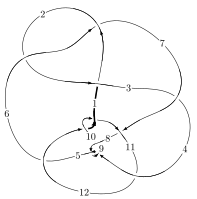
\includegraphics[width=112pt]{../../../GIT/diagram.site/Diagrams/png/1034_12a_0233.png}\\
\ \ \ A knot diagram\footnotemark}&
\allowdisplaybreaks
\textbf{Linearized knot diagam} \\
\cline{2-2}
 &
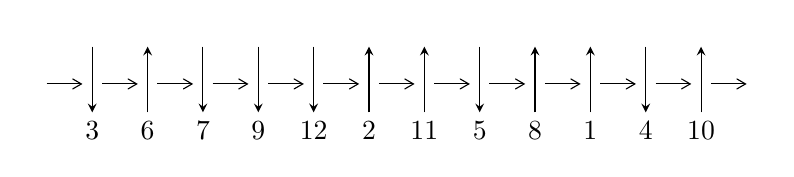
\begin{tikzpicture}[x=20pt, y=17pt]
	% nodes
	\node (C0) at (0, 0) {};
	\node (C1) at (1, 0) {};
	\node (C1U) at (1, +1) {};
	\node (C1D) at (1, -1) {3};

	\node (C2) at (2, 0) {};
	\node (C2U) at (2, +1) {};
	\node (C2D) at (2, -1) {6};

	\node (C3) at (3, 0) {};
	\node (C3U) at (3, +1) {};
	\node (C3D) at (3, -1) {7};

	\node (C4) at (4, 0) {};
	\node (C4U) at (4, +1) {};
	\node (C4D) at (4, -1) {9};

	\node (C5) at (5, 0) {};
	\node (C5U) at (5, +1) {};
	\node (C5D) at (5, -1) {12};

	\node (C6) at (6, 0) {};
	\node (C6U) at (6, +1) {};
	\node (C6D) at (6, -1) {2};

	\node (C7) at (7, 0) {};
	\node (C7U) at (7, +1) {};
	\node (C7D) at (7, -1) {11};

	\node (C8) at (8, 0) {};
	\node (C8U) at (8, +1) {};
	\node (C8D) at (8, -1) {5};

	\node (C9) at (9, 0) {};
	\node (C9U) at (9, +1) {};
	\node (C9D) at (9, -1) {8};

	\node (C10) at (10, 0) {};
	\node (C10U) at (10, +1) {};
	\node (C10D) at (10, -1) {1};

	\node (C11) at (11, 0) {};
	\node (C11U) at (11, +1) {};
	\node (C11D) at (11, -1) {4};

	\node (C12) at (12, 0) {};
	\node (C12U) at (12, +1) {};
	\node (C12D) at (12, -1) {10};
	\node (C13) at (13, 0) {};

	% arrows
	\draw[->,>={angle 60}]
	(C0) edge (C1) (C1) edge (C2) (C2) edge (C3) (C3) edge (C4) (C4) edge (C5) (C5) edge (C6) (C6) edge (C7) (C7) edge (C8) (C8) edge (C9) (C9) edge (C10) (C10) edge (C11) (C11) edge (C12) (C12) edge (C13) ;	\draw[->,>=stealth]
	(C1U) edge (C1D) (C2D) edge (C2U) (C3U) edge (C3D) (C4U) edge (C4D) (C5U) edge (C5D) (C6D) edge (C6U) (C7D) edge (C7U) (C8U) edge (C8D) (C9D) edge (C9U) (C10D) edge (C10U) (C11U) edge (C11D) (C12D) edge (C12U) ;
	\end{tikzpicture} \\
\hhline{~~} \\& 
\textbf{Solving Sequence} \\ \cline{2-2} 
 &
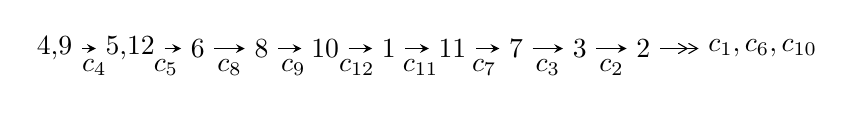
\begin{tikzpicture}[x=23pt, y=7pt]
	% node
	\node (A0) at (-1/8, 0) {4,9};
	\node (A1) at (17/16, 0) {5,12};
	\node (A2) at (17/8, 0) {6};
	\node (A3) at (25/8, 0) {8};
	\node (A4) at (33/8, 0) {10};
	\node (A5) at (41/8, 0) {1};
	\node (A6) at (49/8, 0) {11};
	\node (A7) at (57/8, 0) {7};
	\node (A8) at (65/8, 0) {3};
	\node (A9) at (73/8, 0) {2};
	\node (C1) at (1/2, -1) {$c_{4}$};
	\node (C2) at (13/8, -1) {$c_{5}$};
	\node (C3) at (21/8, -1) {$c_{8}$};
	\node (C4) at (29/8, -1) {$c_{9}$};
	\node (C5) at (37/8, -1) {$c_{12}$};
	\node (C6) at (45/8, -1) {$c_{11}$};
	\node (C7) at (53/8, -1) {$c_{7}$};
	\node (C8) at (61/8, -1) {$c_{3}$};
	\node (C9) at (69/8, -1) {$c_{2}$};
	\node (A10) at (11, 0) {$c_{1},c_{6},c_{10}$};

	% edge
	\draw[->,>=stealth]	
	(A0) edge (A1) (A1) edge (A2) (A2) edge (A3) (A3) edge (A4) (A4) edge (A5) (A5) edge (A6) (A6) edge (A7) (A7) edge (A8) (A8) edge (A9) ;
	\draw[->>,>={angle 60}]	
	(A9) edge (A10);
\end{tikzpicture} \\ 

\end{tabular} \\

\footnotetext{
The image of knot diagram is generated by the software ``\textbf{Draw programme}" developed by Andrew Bartholomew(\url{http://www.layer8.co.uk/maths/draw/index.htm\#Running-draw}), where we modified some parts for our purpose(\url{https://github.com/CATsTAILs/LinksPainter}).
}\phantom \\ \newline 
\centering \textbf{Ideals for irreducible components\footnotemark of $X_{\text{par}}$} 
 
\begin{align*}
I^u_{1}&=\langle 
4.18488\times10^{227} u^{127}+5.48646\times10^{227} u^{126}+\cdots+2.24973\times10^{228} b+1.02313\times10^{228},\\
\phantom{I^u_{1}}&\phantom{= \langle  }1.34465\times10^{228} u^{127}+5.19412\times10^{228} u^{126}+\cdots+7.31163\times10^{228} a+8.12721\times10^{228},\;u^{128}+2 u^{127}+\cdots+4 u+1\rangle \\
I^u_{2}&=\langle 
b,\;21 u^3-14 u^2+13 a+54 u-24,\;u^4- u^3+3 u^2-2 u+1\rangle \\
\\
\end{align*}
\raggedright * 2 irreducible components of $\dim_{\mathbb{C}}=0$, with total 132 representations.\\
\footnotetext{All coefficients of polynomials are rational numbers. But the coefficients are sometimes approximated in decimal forms when there is not enough margin.}
\newpage
\renewcommand{\arraystretch}{1}
\centering \section*{I. $I^u_{1}= \langle 4.18\times10^{227} u^{127}+5.49\times10^{227} u^{126}+\cdots+2.25\times10^{228} b+1.02\times10^{228},\;1.34\times10^{228} u^{127}+5.19\times10^{228} u^{126}+\cdots+7.31\times10^{228} a+8.13\times10^{228},\;u^{128}+2 u^{127}+\cdots+4 u+1 \rangle$}
\flushleft \textbf{(i) Arc colorings}\\
\begin{tabular}{m{7pt} m{180pt} m{7pt} m{180pt} }
\flushright $a_{4}=$&$\begin{pmatrix}1\\0\end{pmatrix}$ \\
\flushright $a_{9}=$&$\begin{pmatrix}0\\u\end{pmatrix}$ \\
\flushright $a_{5}=$&$\begin{pmatrix}1\\u^2\end{pmatrix}$ \\
\flushright $a_{12}=$&$\begin{pmatrix}-0.183906 u^{127}-0.710391 u^{126}+\cdots-2.82573 u-1.11155\\-0.186017 u^{127}-0.243872 u^{126}+\cdots+0.364001 u-0.454777\end{pmatrix}$ \\
\flushright $a_{6}=$&$\begin{pmatrix}2.12621 u^{127}+7.12324 u^{126}+\cdots+18.8467 u+7.04245\\-0.141375 u^{127}-0.0767156 u^{126}+\cdots+0.384787 u+0.310717\end{pmatrix}$ \\
\flushright $a_{8}=$&$\begin{pmatrix}u\\u^3+u\end{pmatrix}$ \\
\flushright $a_{10}=$&$\begin{pmatrix}u^3\\u^5+u^3+u\end{pmatrix}$ \\
\flushright $a_{1}=$&$\begin{pmatrix}-0.0809780 u^{127}-0.414723 u^{126}+\cdots-2.39257 u-0.955381\\u^5+u^3+u\end{pmatrix}$ \\
\flushright $a_{11}=$&$\begin{pmatrix}-0.369923 u^{127}-0.954263 u^{126}+\cdots-2.46172 u-1.56632\\-0.186017 u^{127}-0.243872 u^{126}+\cdots+0.364001 u-0.454777\end{pmatrix}$ \\
\flushright $a_{7}=$&$\begin{pmatrix}-0.272534 u^{127}-4.23409 u^{126}+\cdots-10.9206 u-2.04342\\0.306137 u^{127}+0.382329 u^{126}+\cdots+1.78713 u+0.793514\end{pmatrix}$ \\
\flushright $a_{3}=$&$\begin{pmatrix}-2.12817 u^{127}-3.27752 u^{126}+\cdots-6.67846 u-1.39973\\0.0958762 u^{127}+0.310460 u^{126}+\cdots+2.02656 u+0.685172\end{pmatrix}$ \\
\flushright $a_{2}=$&$\begin{pmatrix}0.289840 u^{127}+0.491603 u^{126}+\cdots+2.31147 u+0.795233\\0.413994 u^{127}+0.479323 u^{126}+\cdots+1.65330 u+0.537177\end{pmatrix}$\\&\end{tabular}
\flushleft \textbf{(ii) Obstruction class $= -1$}\\~\\
\flushleft \textbf{(iii) Cusp Shapes $= 0.987890 u^{127}-5.81033 u^{126}+\cdots-41.3925 u-15.5122$}\\~\\
\newpage\renewcommand{\arraystretch}{1}
\flushleft \textbf{(iv) u-Polynomials at the component}\newline \\
\begin{tabular}{m{50pt}|m{274pt}}
Crossings & \hspace{64pt}u-Polynomials at each crossing \\
\hline $$\begin{aligned}c_{1}\end{aligned}$$&$\begin{aligned}
&u^{128}+62 u^{127}+\cdots+4 u+1
\end{aligned}$\\
\hline $$\begin{aligned}c_{2},c_{6}\end{aligned}$$&$\begin{aligned}
&u^{128}-2 u^{127}+\cdots-2 u+1
\end{aligned}$\\
\hline $$\begin{aligned}c_{3}\end{aligned}$$&$\begin{aligned}
&u^{128}+2 u^{127}+\cdots+4224656 u+1446152
\end{aligned}$\\
\hline $$\begin{aligned}c_{4},c_{8}\end{aligned}$$&$\begin{aligned}
&u^{128}+2 u^{127}+\cdots+4 u+1
\end{aligned}$\\
\hline $$\begin{aligned}c_{5}\end{aligned}$$&$\begin{aligned}
&13(13 u^{128}-13 u^{127}+\cdots-23585 u+12601)
\end{aligned}$\\
\hline $$\begin{aligned}c_{7}\end{aligned}$$&$\begin{aligned}
&13(13 u^{128}+104 u^{127}+\cdots+257066 u+17686)
\end{aligned}$\\
\hline $$\begin{aligned}c_{9}\end{aligned}$$&$\begin{aligned}
&u^{128}-58 u^{127}+\cdots-4 u+1
\end{aligned}$\\
\hline $$\begin{aligned}c_{10},c_{12}\end{aligned}$$&$\begin{aligned}
&u^{128}+5 u^{127}+\cdots+1642 u+169
\end{aligned}$\\
\hline $$\begin{aligned}c_{11}\end{aligned}$$&$\begin{aligned}
&u^{128}+5 u^{127}+\cdots+25272 u+2704
\end{aligned}$\\
\hline
\end{tabular}\\~\\
\newpage\renewcommand{\arraystretch}{1}
\flushleft \textbf{(v) Riley Polynomials at the component}\newline \\
\begin{tabular}{m{50pt}|m{274pt}}
Crossings & \hspace{64pt}Riley Polynomials at each crossing \\
\hline $$\begin{aligned}c_{1}\end{aligned}$$&$\begin{aligned}
&y^{128}+10 y^{127}+\cdots+16 y+1
\end{aligned}$\\
\hline $$\begin{aligned}c_{2},c_{6}\end{aligned}$$&$\begin{aligned}
&y^{128}+62 y^{127}+\cdots+4 y+1
\end{aligned}$\\
\hline $$\begin{aligned}c_{3}\end{aligned}$$&$\begin{aligned}
&y^{128}-42 y^{127}+\cdots-15693533191440 y+2091355607104
\end{aligned}$\\
\hline $$\begin{aligned}c_{4},c_{8}\end{aligned}$$&$\begin{aligned}
&y^{128}+58 y^{127}+\cdots+4 y+1
\end{aligned}$\\
\hline $$\begin{aligned}c_{5}\end{aligned}$$&$\begin{aligned}
&169(169 y^{128}+5603 y^{127}+\cdots-9.11953\times10^{8} y+1.58785\times10^{8})
\end{aligned}$\\
\hline $$\begin{aligned}c_{7}\end{aligned}$$&$\begin{aligned}
&169(169 y^{128}+11180 y^{127}+\cdots+1.65779\times10^{10} y+3.12795\times10^{8})
\end{aligned}$\\
\hline $$\begin{aligned}c_{9}\end{aligned}$$&$\begin{aligned}
&y^{128}+26 y^{127}+\cdots+64 y+1
\end{aligned}$\\
\hline $$\begin{aligned}c_{10},c_{12}\end{aligned}$$&$\begin{aligned}
&y^{128}-75 y^{127}+\cdots+85914 y+28561
\end{aligned}$\\
\hline $$\begin{aligned}c_{11}\end{aligned}$$&$\begin{aligned}
&y^{128}-27 y^{127}+\cdots+238719936 y+7311616
\end{aligned}$\\
\hline
\end{tabular}\\~\\
\newpage\flushleft \textbf{(vi) Complex Volumes and Cusp Shapes}
$$\begin{array}{c|c|c}  
\text{Solutions to }I^u_{1}& \I (\text{vol} + \sqrt{-1}CS) & \text{Cusp shape}\\
 \hline 
\begin{aligned}
u &= -0.632351 + 0.776627 I \\
a &= \phantom{-}0.384670 + 0.174926 I \\
b &= \phantom{-}0.468234 + 0.140402 I\end{aligned}
 & -0.40228 + 1.86126 I & \phantom{-0.000000 } 0 \\ \hline\begin{aligned}
u &= -0.632351 - 0.776627 I \\
a &= \phantom{-}0.384670 - 0.174926 I \\
b &= \phantom{-}0.468234 - 0.140402 I\end{aligned}
 & -0.40228 - 1.86126 I & \phantom{-0.000000 } 0 \\ \hline\begin{aligned}
u &= \phantom{-}0.898979 + 0.430780 I \\
a &= \phantom{-}0.129023 + 0.106373 I \\
b &= \phantom{-}1.16662 - 0.85267 I\end{aligned}
 & -0.07280 + 8.63391 I & \phantom{-0.000000 } 0 \\ \hline\begin{aligned}
u &= \phantom{-}0.898979 - 0.430780 I \\
a &= \phantom{-}0.129023 - 0.106373 I \\
b &= \phantom{-}1.16662 + 0.85267 I\end{aligned}
 & -0.07280 - 8.63391 I & \phantom{-0.000000 } 0 \\ \hline\begin{aligned}
u &= -0.895363 + 0.438019 I \\
a &= -0.156897 + 0.105804 I \\
b &= -1.24502 - 0.90117 I\end{aligned}
 & -2.65354 - 13.84350 I & \phantom{-0.000000 } 0 \\ \hline\begin{aligned}
u &= -0.895363 - 0.438019 I \\
a &= -0.156897 - 0.105804 I \\
b &= -1.24502 + 0.90117 I\end{aligned}
 & -2.65354 + 13.84350 I & \phantom{-0.000000 } 0 \\ \hline\begin{aligned}
u &= \phantom{-}0.929547 + 0.405477 I \\
a &= \phantom{-}0.0413716 + 0.0807925 I \\
b &= \phantom{-}0.848325 - 0.738830 I\end{aligned}
 & \phantom{-}2.38568 + 6.03387 I & \phantom{-0.000000 } 0 \\ \hline\begin{aligned}
u &= \phantom{-}0.929547 - 0.405477 I \\
a &= \phantom{-}0.0413716 - 0.0807925 I \\
b &= \phantom{-}0.848325 + 0.738830 I\end{aligned}
 & \phantom{-}2.38568 - 6.03387 I & \phantom{-0.000000 } 0 \\ \hline\begin{aligned}
u &= -0.885131 + 0.421262 I \\
a &= -0.115650 + 0.156423 I \\
b &= -1.221290 - 0.694121 I\end{aligned}
 & -4.91627 - 5.37289 I & \phantom{-0.000000 } 0 \\ \hline\begin{aligned}
u &= -0.885131 - 0.421262 I \\
a &= -0.115650 - 0.156423 I \\
b &= -1.221290 + 0.694121 I\end{aligned}
 & -4.91627 + 5.37289 I & \phantom{-0.000000 } 0\\
 \hline 
 \end{array}$$\newpage$$\begin{array}{c|c|c}  
\text{Solutions to }I^u_{1}& \I (\text{vol} + \sqrt{-1}CS) & \text{Cusp shape}\\
 \hline 
\begin{aligned}
u &= -0.952929 + 0.376629 I \\
a &= \phantom{-}0.0036938 + 0.0791327 I \\
b &= -0.702715 - 0.596805 I\end{aligned}
 & \phantom{-}2.00855 - 0.71097 I & \phantom{-0.000000 } 0 \\ \hline\begin{aligned}
u &= -0.952929 - 0.376629 I \\
a &= \phantom{-}0.0036938 - 0.0791327 I \\
b &= -0.702715 + 0.596805 I\end{aligned}
 & \phantom{-}2.00855 + 0.71097 I & \phantom{-0.000000 } 0 \\ \hline\begin{aligned}
u &= \phantom{-}0.818015 + 0.622461 I \\
a &= -0.186819 + 0.231456 I \\
b &= -1.110050 - 0.108095 I\end{aligned}
 & -6.18849 - 1.43861 I & \phantom{-0.000000 } 0 \\ \hline\begin{aligned}
u &= \phantom{-}0.818015 - 0.622461 I \\
a &= -0.186819 - 0.231456 I \\
b &= -1.110050 + 0.108095 I\end{aligned}
 & -6.18849 + 1.43861 I & \phantom{-0.000000 } 0 \\ \hline\begin{aligned}
u &= -0.274045 + 0.926878 I \\
a &= -0.92575 - 2.27337 I \\
b &= -0.602160 + 1.228960 I\end{aligned}
 & \phantom{-}1.73156 + 2.55640 I & \phantom{-0.000000 } 0 \\ \hline\begin{aligned}
u &= -0.274045 - 0.926878 I \\
a &= -0.92575 + 2.27337 I \\
b &= -0.602160 - 1.228960 I\end{aligned}
 & \phantom{-}1.73156 - 2.55640 I & \phantom{-0.000000 } 0 \\ \hline\begin{aligned}
u &= -0.322986 + 0.983840 I \\
a &= -0.41115 - 2.42512 I \\
b &= -1.34793 + 1.14806 I\end{aligned}
 & \phantom{-}2.69083 - 3.89242 I & \phantom{-0.000000 } 0 \\ \hline\begin{aligned}
u &= -0.322986 - 0.983840 I \\
a &= -0.41115 + 2.42512 I \\
b &= -1.34793 - 1.14806 I\end{aligned}
 & \phantom{-}2.69083 + 3.89242 I & \phantom{-0.000000 } 0 \\ \hline\begin{aligned}
u &= \phantom{-}0.346007 + 0.977002 I \\
a &= \phantom{-}0.31122 - 2.15276 I \\
b &= \phantom{-}1.36159 + 0.83379 I\end{aligned}
 & \phantom{-}4.67825 - 0.54660 I & \phantom{-0.000000 } 0 \\ \hline\begin{aligned}
u &= \phantom{-}0.346007 - 0.977002 I \\
a &= \phantom{-}0.31122 + 2.15276 I \\
b &= \phantom{-}1.36159 - 0.83379 I\end{aligned}
 & \phantom{-}4.67825 + 0.54660 I & \phantom{-0.000000 } 0\\
 \hline 
 \end{array}$$\newpage$$\begin{array}{c|c|c}  
\text{Solutions to }I^u_{1}& \I (\text{vol} + \sqrt{-1}CS) & \text{Cusp shape}\\
 \hline 
\begin{aligned}
u &= -0.426686 + 0.862947 I \\
a &= -2.03486 - 3.06355 I \\
b &= -0.329659 + 0.305677 I\end{aligned}
 & \phantom{-}1.78616 + 1.80735 I & \phantom{-0.000000 } 0 \\ \hline\begin{aligned}
u &= -0.426686 - 0.862947 I \\
a &= -2.03486 + 3.06355 I \\
b &= -0.329659 - 0.305677 I\end{aligned}
 & \phantom{-}1.78616 - 1.80735 I & \phantom{-0.000000 } 0 \\ \hline\begin{aligned}
u &= \phantom{-}0.526025 + 0.894900 I \\
a &= -3.64824 + 6.31543 I \\
b &= -0.057519 - 0.285480 I\end{aligned}
 & -0.91250 + 1.67927 I & \phantom{-0.000000 } 0 \\ \hline\begin{aligned}
u &= \phantom{-}0.526025 - 0.894900 I \\
a &= -3.64824 - 6.31543 I \\
b &= -0.057519 + 0.285480 I\end{aligned}
 & -0.91250 - 1.67927 I & \phantom{-0.000000 } 0 \\ \hline\begin{aligned}
u &= -0.500220 + 0.917179 I \\
a &= -0.90698 + 3.81295 I \\
b &= -0.208222 - 0.324824 I\end{aligned}
 & \phantom{-}1.63645 + 2.27841 I & \phantom{-0.000000 } 0 \\ \hline\begin{aligned}
u &= -0.500220 - 0.917179 I \\
a &= -0.90698 - 3.81295 I \\
b &= -0.208222 + 0.324824 I\end{aligned}
 & \phantom{-}1.63645 - 2.27841 I & \phantom{-0.000000 } 0 \\ \hline\begin{aligned}
u &= \phantom{-}0.384306 + 0.990713 I \\
a &= -0.11804 - 1.66145 I \\
b &= \phantom{-}1.57928 + 0.30620 I\end{aligned}
 & \phantom{-}4.93867 - 1.81136 I & \phantom{-0.000000 } 0 \\ \hline\begin{aligned}
u &= \phantom{-}0.384306 - 0.990713 I \\
a &= -0.11804 + 1.66145 I \\
b &= \phantom{-}1.57928 - 0.30620 I\end{aligned}
 & \phantom{-}4.93867 + 1.81136 I & \phantom{-0.000000 } 0 \\ \hline\begin{aligned}
u &= -0.037841 + 0.932887 I \\
a &= -1.66931 - 1.32141 I \\
b &= \phantom{-}0.613399 + 1.108330 I\end{aligned}
 & -0.95705 - 6.55438 I & \phantom{-0.000000 } 0 \\ \hline\begin{aligned}
u &= -0.037841 - 0.932887 I \\
a &= -1.66931 + 1.32141 I \\
b &= \phantom{-}0.613399 - 1.108330 I\end{aligned}
 & -0.95705 + 6.55438 I & \phantom{-0.000000 } 0\\
 \hline 
 \end{array}$$\newpage$$\begin{array}{c|c|c}  
\text{Solutions to }I^u_{1}& \I (\text{vol} + \sqrt{-1}CS) & \text{Cusp shape}\\
 \hline 
\begin{aligned}
u &= \phantom{-}0.535878 + 0.927976 I \\
a &= -2.05775 + 2.73591 I \\
b &= \phantom{-}0.015290 - 0.533756 I\end{aligned}
 & -1.26429 - 5.66383 I & \phantom{-0.000000 } 0 \\ \hline\begin{aligned}
u &= \phantom{-}0.535878 - 0.927976 I \\
a &= -2.05775 - 2.73591 I \\
b &= \phantom{-}0.015290 + 0.533756 I\end{aligned}
 & -1.26429 + 5.66383 I & \phantom{-0.000000 } 0 \\ \hline\begin{aligned}
u &= -0.745382 + 0.545622 I \\
a &= \phantom{-}0.077721 + 0.386047 I \\
b &= \phantom{-}1.42048 + 0.54522 I\end{aligned}
 & -7.27264 + 0.58083 I & \phantom{-0.000000 } 0 \\ \hline\begin{aligned}
u &= -0.745382 - 0.545622 I \\
a &= \phantom{-}0.077721 - 0.386047 I \\
b &= \phantom{-}1.42048 - 0.54522 I\end{aligned}
 & -7.27264 - 0.58083 I & \phantom{-0.000000 } 0 \\ \hline\begin{aligned}
u &= \phantom{-}0.883502 + 0.625066 I \\
a &= -0.191745 + 0.163487 I \\
b &= -0.948287 - 0.428041 I\end{aligned}
 & -3.74142 - 9.48538 I & \phantom{-0.000000 } 0 \\ \hline\begin{aligned}
u &= \phantom{-}0.883502 - 0.625066 I \\
a &= -0.191745 - 0.163487 I \\
b &= -0.948287 + 0.428041 I\end{aligned}
 & -3.74142 + 9.48538 I & \phantom{-0.000000 } 0 \\ \hline\begin{aligned}
u &= -0.400087 + 1.007720 I \\
a &= \phantom{-}0.57220 - 1.45592 I \\
b &= -1.80895 - 0.00572 I\end{aligned}
 & \phantom{-}3.23788 + 6.12295 I & \phantom{-0.000000 } 0 \\ \hline\begin{aligned}
u &= -0.400087 - 1.007720 I \\
a &= \phantom{-}0.57220 + 1.45592 I \\
b &= -1.80895 + 0.00572 I\end{aligned}
 & \phantom{-}3.23788 - 6.12295 I & \phantom{-0.000000 } 0 \\ \hline\begin{aligned}
u &= -0.873555 + 0.658407 I \\
a &= \phantom{-}0.163345 + 0.182698 I \\
b &= \phantom{-}0.860741 - 0.290075 I\end{aligned}
 & -1.37571 + 4.26938 I & \phantom{-0.000000 } 0 \\ \hline\begin{aligned}
u &= -0.873555 - 0.658407 I \\
a &= \phantom{-}0.163345 - 0.182698 I \\
b &= \phantom{-}0.860741 + 0.290075 I\end{aligned}
 & -1.37571 - 4.26938 I & \phantom{-0.000000 } 0\\
 \hline 
 \end{array}$$\newpage$$\begin{array}{c|c|c}  
\text{Solutions to }I^u_{1}& \I (\text{vol} + \sqrt{-1}CS) & \text{Cusp shape}\\
 \hline 
\begin{aligned}
u &= \phantom{-}0.096379 + 0.890392 I \\
a &= -1.36267 - 0.83058 I \\
b &= \phantom{-}0.566969 + 0.647022 I\end{aligned}
 & -2.01309 + 1.15458 I & \phantom{-0.000000 } 0 \\ \hline\begin{aligned}
u &= \phantom{-}0.096379 - 0.890392 I \\
a &= -1.36267 + 0.83058 I \\
b &= \phantom{-}0.566969 - 0.647022 I\end{aligned}
 & -2.01309 - 1.15458 I & \phantom{-0.000000 } 0 \\ \hline\begin{aligned}
u &= \phantom{-}0.718201 + 0.533561 I \\
a &= \phantom{-}0.019695 + 0.390470 I \\
b &= -1.30885 + 0.75980 I\end{aligned}
 & -3.18770 + 2.76839 I & \phantom{-0.000000 } 0 \\ \hline\begin{aligned}
u &= \phantom{-}0.718201 - 0.533561 I \\
a &= \phantom{-}0.019695 - 0.390470 I \\
b &= -1.30885 - 0.75980 I\end{aligned}
 & -3.18770 - 2.76839 I & \phantom{-0.000000 } 0 \\ \hline\begin{aligned}
u &= -0.727223 + 0.517544 I \\
a &= -0.015327 + 0.459392 I \\
b &= \phantom{-}1.44559 + 0.83679 I\end{aligned}
 & -5.85757 - 7.54109 I & \phantom{-0.000000 } 0 \\ \hline\begin{aligned}
u &= -0.727223 - 0.517544 I \\
a &= -0.015327 - 0.459392 I \\
b &= \phantom{-}1.44559 - 0.83679 I\end{aligned}
 & -5.85757 + 7.54109 I & \phantom{-0.000000 } 0 \\ \hline\begin{aligned}
u &= \phantom{-}0.200788 + 0.867511 I \\
a &= \phantom{-}1.08886 - 1.93715 I \\
b &= \phantom{-}0.099058 + 1.157480 I\end{aligned}
 & \phantom{-}2.81820 + 1.20231 I & \phantom{-0.000000 } 0 \\ \hline\begin{aligned}
u &= \phantom{-}0.200788 - 0.867511 I \\
a &= \phantom{-}1.08886 + 1.93715 I \\
b &= \phantom{-}0.099058 - 1.157480 I\end{aligned}
 & \phantom{-}2.81820 - 1.20231 I & \phantom{-0.000000 } 0 \\ \hline\begin{aligned}
u &= \phantom{-}0.492212 + 0.740960 I \\
a &= -2.20367 - 1.81776 I \\
b &= -0.101543 + 0.598383 I\end{aligned}
 & -1.38202 - 5.91758 I & \phantom{-0.000000 } 0 \\ \hline\begin{aligned}
u &= \phantom{-}0.492212 - 0.740960 I \\
a &= -2.20367 + 1.81776 I \\
b &= -0.101543 - 0.598383 I\end{aligned}
 & -1.38202 + 5.91758 I & \phantom{-0.000000 } 0\\
 \hline 
 \end{array}$$\newpage$$\begin{array}{c|c|c}  
\text{Solutions to }I^u_{1}& \I (\text{vol} + \sqrt{-1}CS) & \text{Cusp shape}\\
 \hline 
\begin{aligned}
u &= -0.448235 + 1.016420 I \\
a &= \phantom{-}1.120110 - 0.326616 I \\
b &= -1.52198 - 0.89095 I\end{aligned}
 & \phantom{-}2.92272 + 0.14341 I & \phantom{-0.000000 } 0 \\ \hline\begin{aligned}
u &= -0.448235 - 1.016420 I \\
a &= \phantom{-}1.120110 + 0.326616 I \\
b &= -1.52198 + 0.89095 I\end{aligned}
 & \phantom{-}2.92272 - 0.14341 I & \phantom{-0.000000 } 0 \\ \hline\begin{aligned}
u &= \phantom{-}0.471306 + 1.015550 I \\
a &= -1.220560 + 0.267213 I \\
b &= \phantom{-}1.16705 - 1.18281 I\end{aligned}
 & \phantom{-}4.35010 - 4.32900 I & \phantom{-0.000000 } 0 \\ \hline\begin{aligned}
u &= \phantom{-}0.471306 - 1.015550 I \\
a &= -1.220560 - 0.267213 I \\
b &= \phantom{-}1.16705 + 1.18281 I\end{aligned}
 & \phantom{-}4.35010 + 4.32900 I & \phantom{-0.000000 } 0 \\ \hline\begin{aligned}
u &= \phantom{-}0.054445 + 0.874045 I \\
a &= \phantom{-}1.38644 - 1.39055 I \\
b &= -0.390969 + 1.030140 I\end{aligned}
 & \phantom{-}1.56973 + 2.00866 I & \phantom{-0.000000 } 0 \\ \hline\begin{aligned}
u &= \phantom{-}0.054445 - 0.874045 I \\
a &= \phantom{-}1.38644 + 1.39055 I \\
b &= -0.390969 - 1.030140 I\end{aligned}
 & \phantom{-}1.56973 - 2.00866 I & \phantom{-0.000000 } 0 \\ \hline\begin{aligned}
u &= -0.449444 + 0.749502 I \\
a &= \phantom{-}1.16998 - 2.30692 I \\
b &= -0.000337 + 0.566212 I\end{aligned}
 & \phantom{-}1.08929 + 1.73625 I & \phantom{-0.000000 } 0 \\ \hline\begin{aligned}
u &= -0.449444 - 0.749502 I \\
a &= \phantom{-}1.16998 + 2.30692 I \\
b &= -0.000337 - 0.566212 I\end{aligned}
 & \phantom{-}1.08929 - 1.73625 I & \phantom{-0.000000 } 0 \\ \hline\begin{aligned}
u &= -0.578952 + 0.966012 I \\
a &= \phantom{-}0.95852 + 1.19777 I \\
b &= \phantom{-}0.373143 - 0.693459 I\end{aligned}
 & \phantom{-}0.30632 + 2.86178 I & \phantom{-0.000000 } 0 \\ \hline\begin{aligned}
u &= -0.578952 - 0.966012 I \\
a &= \phantom{-}0.95852 - 1.19777 I \\
b &= \phantom{-}0.373143 + 0.693459 I\end{aligned}
 & \phantom{-}0.30632 - 2.86178 I & \phantom{-0.000000 } 0\\
 \hline 
 \end{array}$$\newpage$$\begin{array}{c|c|c}  
\text{Solutions to }I^u_{1}& \I (\text{vol} + \sqrt{-1}CS) & \text{Cusp shape}\\
 \hline 
\begin{aligned}
u &= \phantom{-}0.793240 + 0.356284 I \\
a &= -0.107941 + 0.280203 I \\
b &= \phantom{-}1.071670 - 0.042848 I\end{aligned}
 & -6.33619 + 3.32794 I & \phantom{-0.000000 } 0 \\ \hline\begin{aligned}
u &= \phantom{-}0.793240 - 0.356284 I \\
a &= -0.107941 - 0.280203 I \\
b &= \phantom{-}1.071670 + 0.042848 I\end{aligned}
 & -6.33619 - 3.32794 I & \phantom{-0.000000 } 0 \\ \hline\begin{aligned}
u &= \phantom{-}0.497702 + 1.025980 I \\
a &= -1.52817 + 0.84837 I \\
b &= \phantom{-}0.77404 - 1.61636 I\end{aligned}
 & \phantom{-}3.64882 - 5.60532 I & \phantom{-0.000000 } 0 \\ \hline\begin{aligned}
u &= \phantom{-}0.497702 - 1.025980 I \\
a &= -1.52817 - 0.84837 I \\
b &= \phantom{-}0.77404 + 1.61636 I\end{aligned}
 & \phantom{-}3.64882 + 5.60532 I & \phantom{-0.000000 } 0 \\ \hline\begin{aligned}
u &= -0.528951 + 1.014510 I \\
a &= \phantom{-}1.29255 + 1.35472 I \\
b &= -0.12714 - 1.48116 I\end{aligned}
 & \phantom{-}0.08476 + 3.28264 I & \phantom{-0.000000 } 0 \\ \hline\begin{aligned}
u &= -0.528951 - 1.014510 I \\
a &= \phantom{-}1.29255 - 1.35472 I \\
b &= -0.12714 + 1.48116 I\end{aligned}
 & \phantom{-}0.08476 - 3.28264 I & \phantom{-0.000000 } 0 \\ \hline\begin{aligned}
u &= \phantom{-}0.630037 + 0.571249 I \\
a &= \phantom{-}0.119204 + 0.091100 I \\
b &= -0.731769 + 0.766308 I\end{aligned}
 & -1.01345 + 1.95971 I & \phantom{-0.000000 } 0 \\ \hline\begin{aligned}
u &= \phantom{-}0.630037 - 0.571249 I \\
a &= \phantom{-}0.119204 - 0.091100 I \\
b &= -0.731769 - 0.766308 I\end{aligned}
 & -1.01345 - 1.95971 I & \phantom{-0.000000 } 0 \\ \hline\begin{aligned}
u &= -0.504744 + 1.035910 I \\
a &= \phantom{-}1.72928 + 1.01611 I \\
b &= -0.67860 - 1.87767 I\end{aligned}
 & \phantom{-}1.48535 + 10.17420 I & \phantom{-0.000000 } 0 \\ \hline\begin{aligned}
u &= -0.504744 - 1.035910 I \\
a &= \phantom{-}1.72928 - 1.01611 I \\
b &= -0.67860 + 1.87767 I\end{aligned}
 & \phantom{-}1.48535 - 10.17420 I & \phantom{-0.000000 } 0\\
 \hline 
 \end{array}$$\newpage$$\begin{array}{c|c|c}  
\text{Solutions to }I^u_{1}& \I (\text{vol} + \sqrt{-1}CS) & \text{Cusp shape}\\
 \hline 
\begin{aligned}
u &= \phantom{-}0.464624 + 0.685655 I \\
a &= -1.27292 - 0.93048 I \\
b &= \phantom{-}0.025724 + 0.647128 I\end{aligned}
 & -1.99473 + 1.41613 I & \phantom{-0.000000 } 0 \\ \hline\begin{aligned}
u &= \phantom{-}0.464624 - 0.685655 I \\
a &= -1.27292 + 0.93048 I \\
b &= \phantom{-}0.025724 - 0.647128 I\end{aligned}
 & -1.99473 - 1.41613 I & \phantom{-0.000000 } 0 \\ \hline\begin{aligned}
u &= \phantom{-}0.589028 + 1.017350 I \\
a &= -0.78540 + 1.70504 I \\
b &= -0.83917 - 1.14462 I\end{aligned}
 & \phantom{-}0.31608 - 6.78721 I & \phantom{-0.000000 } 0 \\ \hline\begin{aligned}
u &= \phantom{-}0.589028 - 1.017350 I \\
a &= -0.78540 - 1.70504 I \\
b &= -0.83917 + 1.14462 I\end{aligned}
 & \phantom{-}0.31608 + 6.78721 I & \phantom{-0.000000 } 0 \\ \hline\begin{aligned}
u &= \phantom{-}0.707936 + 0.362323 I \\
a &= -0.275552 + 0.323362 I \\
b &= \phantom{-}0.974206 + 0.241415 I\end{aligned}
 & -5.25090 - 5.17198 I & \phantom{-0.000000 } 0 \\ \hline\begin{aligned}
u &= \phantom{-}0.707936 - 0.362323 I \\
a &= -0.275552 - 0.323362 I \\
b &= \phantom{-}0.974206 - 0.241415 I\end{aligned}
 & -5.25090 + 5.17198 I & \phantom{-0.000000 } 0 \\ \hline\begin{aligned}
u &= -0.760118 + 0.936366 I \\
a &= \phantom{-}0.003216 + 0.528381 I \\
b &= \phantom{-}0.672054 + 0.027651 I\end{aligned}
 & -0.49600 + 1.69688 I & \phantom{-0.000000 } 0 \\ \hline\begin{aligned}
u &= -0.760118 - 0.936366 I \\
a &= \phantom{-}0.003216 - 0.528381 I \\
b &= \phantom{-}0.672054 - 0.027651 I\end{aligned}
 & -0.49600 - 1.69688 I & \phantom{-0.000000 } 0 \\ \hline\begin{aligned}
u &= -0.734325 + 0.300986 I \\
a &= \phantom{-}0.224525 + 0.220536 I \\
b &= -0.872585 + 0.091595 I\end{aligned}
 & -2.28361 + 0.47581 I & \phantom{-0.000000 } 0 \\ \hline\begin{aligned}
u &= -0.734325 - 0.300986 I \\
a &= \phantom{-}0.224525 - 0.220536 I \\
b &= -0.872585 - 0.091595 I\end{aligned}
 & -2.28361 - 0.47581 I & \phantom{-0.000000 } 0\\
 \hline 
 \end{array}$$\newpage$$\begin{array}{c|c|c}  
\text{Solutions to }I^u_{1}& \I (\text{vol} + \sqrt{-1}CS) & \text{Cusp shape}\\
 \hline 
\begin{aligned}
u &= \phantom{-}0.610855 + 1.041230 I \\
a &= -0.40502 + 2.02467 I \\
b &= -1.41825 - 1.06966 I\end{aligned}
 & -1.68060 - 7.86822 I & \phantom{-0.000000 } 0 \\ \hline\begin{aligned}
u &= \phantom{-}0.610855 - 1.041230 I \\
a &= -0.40502 - 2.02467 I \\
b &= -1.41825 + 1.06966 I\end{aligned}
 & -1.68060 + 7.86822 I & \phantom{-0.000000 } 0 \\ \hline\begin{aligned}
u &= -0.625131 + 1.041040 I \\
a &= \phantom{-}0.16613 + 1.93058 I \\
b &= \phantom{-}1.50137 - 0.80100 I\end{aligned}
 & -5.79503 + 4.63683 I & \phantom{-0.000000 } 0 \\ \hline\begin{aligned}
u &= -0.625131 - 1.041040 I \\
a &= \phantom{-}0.16613 - 1.93058 I \\
b &= \phantom{-}1.50137 + 0.80100 I\end{aligned}
 & -5.79503 - 4.63683 I & \phantom{-0.000000 } 0 \\ \hline\begin{aligned}
u &= -0.611400 + 1.049250 I \\
a &= \phantom{-}0.35391 + 2.17037 I \\
b &= \phantom{-}1.58312 - 1.12574 I\end{aligned}
 & -4.28254 + 12.66350 I & \phantom{-0.000000 } 0 \\ \hline\begin{aligned}
u &= -0.611400 - 1.049250 I \\
a &= \phantom{-}0.35391 - 2.17037 I \\
b &= \phantom{-}1.58312 + 1.12574 I\end{aligned}
 & -4.28254 - 12.66350 I & \phantom{-0.000000 } 0 \\ \hline\begin{aligned}
u &= \phantom{-}0.679144 + 1.007210 I \\
a &= \phantom{-}0.086544 + 1.125410 I \\
b &= -1.051820 - 0.135293 I\end{aligned}
 & -5.02581 - 4.14807 I & \phantom{-0.000000 } 0 \\ \hline\begin{aligned}
u &= \phantom{-}0.679144 - 1.007210 I \\
a &= \phantom{-}0.086544 - 1.125410 I \\
b &= -1.051820 + 0.135293 I\end{aligned}
 & -5.02581 + 4.14807 I & \phantom{-0.000000 } 0 \\ \hline\begin{aligned}
u &= -0.065310 + 1.260480 I \\
a &= \phantom{-}1.10987 + 1.17405 I \\
b &= -0.904424 - 0.933478 I\end{aligned}
 & \phantom{-}3.43285 - 11.15210 I & \phantom{-0.000000 } 0 \\ \hline\begin{aligned}
u &= -0.065310 - 1.260480 I \\
a &= \phantom{-}1.10987 - 1.17405 I \\
b &= -0.904424 + 0.933478 I\end{aligned}
 & \phantom{-}3.43285 + 11.15210 I & \phantom{-0.000000 } 0\\
 \hline 
 \end{array}$$\newpage$$\begin{array}{c|c|c}  
\text{Solutions to }I^u_{1}& \I (\text{vol} + \sqrt{-1}CS) & \text{Cusp shape}\\
 \hline 
\begin{aligned}
u &= -0.101203 + 1.262340 I \\
a &= \phantom{-}1.072270 + 0.805770 I \\
b &= -0.831818 - 0.644666 I\end{aligned}
 & \phantom{-}0.97764 - 2.56762 I & \phantom{-0.000000 } 0 \\ \hline\begin{aligned}
u &= -0.101203 - 1.262340 I \\
a &= \phantom{-}1.072270 - 0.805770 I \\
b &= -0.831818 + 0.644666 I\end{aligned}
 & \phantom{-}0.97764 + 2.56762 I & \phantom{-0.000000 } 0 \\ \hline\begin{aligned}
u &= \phantom{-}0.763272 + 1.016450 I \\
a &= \phantom{-}0.302516 + 0.578936 I \\
b &= -0.761657 + 0.212115 I\end{aligned}
 & -2.57086 + 3.46847 I & \phantom{-0.000000 } 0 \\ \hline\begin{aligned}
u &= \phantom{-}0.763272 - 1.016450 I \\
a &= \phantom{-}0.302516 - 0.578936 I \\
b &= -0.761657 - 0.212115 I\end{aligned}
 & -2.57086 - 3.46847 I & \phantom{-0.000000 } 0 \\ \hline\begin{aligned}
u &= \phantom{-}0.071409 + 1.271830 I \\
a &= -0.97930 + 1.09070 I \\
b &= \phantom{-}0.789462 - 0.879460 I\end{aligned}
 & \phantom{-}6.01140 + 5.85590 I & \phantom{-0.000000 } 0 \\ \hline\begin{aligned}
u &= \phantom{-}0.071409 - 1.271830 I \\
a &= -0.97930 - 1.09070 I \\
b &= \phantom{-}0.789462 + 0.879460 I\end{aligned}
 & \phantom{-}6.01140 - 5.85590 I & \phantom{-0.000000 } 0 \\ \hline\begin{aligned}
u &= \phantom{-}0.528327 + 1.163720 I \\
a &= -0.728580 - 0.906768 I \\
b &= \phantom{-}0.746221 + 0.117323 I\end{aligned}
 & -2.85021 + 0.40649 I & \phantom{-0.000000 } 0 \\ \hline\begin{aligned}
u &= \phantom{-}0.528327 - 1.163720 I \\
a &= -0.728580 + 0.906768 I \\
b &= \phantom{-}0.746221 - 0.117323 I\end{aligned}
 & -2.85021 - 0.40649 I & \phantom{-0.000000 } 0 \\ \hline\begin{aligned}
u &= \phantom{-}0.594955 + 1.152750 I \\
a &= -0.41766 - 1.37163 I \\
b &= \phantom{-}0.959140 + 0.350193 I\end{aligned}
 & -3.95846 - 8.56048 I & \phantom{-0.000000 } 0 \\ \hline\begin{aligned}
u &= \phantom{-}0.594955 - 1.152750 I \\
a &= -0.41766 + 1.37163 I \\
b &= \phantom{-}0.959140 - 0.350193 I\end{aligned}
 & -3.95846 + 8.56048 I & \phantom{-0.000000 } 0\\
 \hline 
 \end{array}$$\newpage$$\begin{array}{c|c|c}  
\text{Solutions to }I^u_{1}& \I (\text{vol} + \sqrt{-1}CS) & \text{Cusp shape}\\
 \hline 
\begin{aligned}
u &= -0.643161 + 1.137780 I \\
a &= -0.21745 - 1.93403 I \\
b &= -1.26228 + 0.86867 I\end{aligned}
 & -2.75261 + 11.00610 I & \phantom{-0.000000 } 0 \\ \hline\begin{aligned}
u &= -0.643161 - 1.137780 I \\
a &= -0.21745 + 1.93403 I \\
b &= -1.26228 - 0.86867 I\end{aligned}
 & -2.75261 - 11.00610 I & \phantom{-0.000000 } 0 \\ \hline\begin{aligned}
u &= -0.651207 + 1.135620 I \\
a &= -0.42713 - 2.03646 I \\
b &= -1.31308 + 1.04434 I\end{aligned}
 & -0.5375 + 19.5357 I & \phantom{-0.000000 } 0 \\ \hline\begin{aligned}
u &= -0.651207 - 1.135620 I \\
a &= -0.42713 + 2.03646 I \\
b &= -1.31308 - 1.04434 I\end{aligned}
 & -0.5375 - 19.5357 I & \phantom{-0.000000 } 0 \\ \hline\begin{aligned}
u &= \phantom{-}0.650004 + 1.138880 I \\
a &= \phantom{-}0.40382 - 1.93633 I \\
b &= \phantom{-}1.23809 + 1.01206 I\end{aligned}
 & \phantom{-}2.0745 - 14.3290 I & \phantom{-0.000000 } 0 \\ \hline\begin{aligned}
u &= \phantom{-}0.650004 - 1.138880 I \\
a &= \phantom{-}0.40382 + 1.93633 I \\
b &= \phantom{-}1.23809 - 1.01206 I\end{aligned}
 & \phantom{-}2.0745 + 14.3290 I & \phantom{-0.000000 } 0 \\ \hline\begin{aligned}
u &= -0.575489 + 1.189130 I \\
a &= \phantom{-}0.389298 - 1.000600 I \\
b &= -0.736345 + 0.304703 I\end{aligned}
 & \phantom{-}0.38762 + 4.55179 I & \phantom{-0.000000 } 0 \\ \hline\begin{aligned}
u &= -0.575489 - 1.189130 I \\
a &= \phantom{-}0.389298 + 1.000600 I \\
b &= -0.736345 - 0.304703 I\end{aligned}
 & \phantom{-}0.38762 - 4.55179 I & \phantom{-0.000000 } 0 \\ \hline\begin{aligned}
u &= \phantom{-}0.651021 + 1.154090 I \\
a &= \phantom{-}0.41737 - 1.56021 I \\
b &= \phantom{-}0.946995 + 0.959821 I\end{aligned}
 & \phantom{-}4.66018 - 11.80060 I & \phantom{-0.000000 } 0 \\ \hline\begin{aligned}
u &= \phantom{-}0.651021 - 1.154090 I \\
a &= \phantom{-}0.41737 + 1.56021 I \\
b &= \phantom{-}0.946995 - 0.959821 I\end{aligned}
 & \phantom{-}4.66018 + 11.80060 I & \phantom{-0.000000 } 0\\
 \hline 
 \end{array}$$\newpage$$\begin{array}{c|c|c}  
\text{Solutions to }I^u_{1}& \I (\text{vol} + \sqrt{-1}CS) & \text{Cusp shape}\\
 \hline 
\begin{aligned}
u &= -0.649273 + 1.165840 I \\
a &= -0.340607 - 1.351870 I \\
b &= -0.806556 + 0.860138 I\end{aligned}
 & \phantom{-}4.40266 + 6.51601 I & \phantom{-0.000000 } 0 \\ \hline\begin{aligned}
u &= -0.649273 - 1.165840 I \\
a &= -0.340607 + 1.351870 I \\
b &= -0.806556 - 0.860138 I\end{aligned}
 & \phantom{-}4.40266 - 6.51601 I & \phantom{-0.000000 } 0 \\ \hline\begin{aligned}
u &= \phantom{-}0.051760 + 1.351390 I \\
a &= -0.323387 + 0.865265 I \\
b &= \phantom{-}0.256174 - 0.739354 I\end{aligned}
 & \phantom{-}8.69485 + 2.85046 I & \phantom{-0.000000 } 0 \\ \hline\begin{aligned}
u &= \phantom{-}0.051760 - 1.351390 I \\
a &= -0.323387 - 0.865265 I \\
b &= \phantom{-}0.256174 + 0.739354 I\end{aligned}
 & \phantom{-}8.69485 - 2.85046 I & \phantom{-0.000000 } 0 \\ \hline\begin{aligned}
u &= -0.485376 + 0.423733 I \\
a &= -1.006980 - 0.316764 I \\
b &= \phantom{-}0.020564 + 1.180970 I\end{aligned}
 & -1.48749 + 0.97090 I & -3.81000 - 0.30668 I \\ \hline\begin{aligned}
u &= -0.485376 - 0.423733 I \\
a &= -1.006980 + 0.316764 I \\
b &= \phantom{-}0.020564 - 1.180970 I\end{aligned}
 & -1.48749 - 0.97090 I & -3.81000 + 0.30668 I \\ \hline\begin{aligned}
u &= -0.480842 + 0.307056 I \\
a &= -1.66540 - 0.20548 I \\
b &= -0.439562 + 1.314170 I\end{aligned}
 & -0.38770 - 6.08787 I & -1.35496 + 6.52586 I \\ \hline\begin{aligned}
u &= -0.480842 - 0.307056 I \\
a &= -1.66540 + 0.20548 I \\
b &= -0.439562 - 1.314170 I\end{aligned}
 & -0.38770 + 6.08787 I & -1.35496 - 6.52586 I \\ \hline\begin{aligned}
u &= \phantom{-}0.421069 + 0.301666 I \\
a &= \phantom{-}1.75107 - 0.54964 I \\
b &= \phantom{-}0.443775 + 1.063820 I\end{aligned}
 & \phantom{-}1.85296 + 1.65232 I & \phantom{-}2.94839 - 2.48371 I \\ \hline\begin{aligned}
u &= \phantom{-}0.421069 - 0.301666 I \\
a &= \phantom{-}1.75107 + 0.54964 I \\
b &= \phantom{-}0.443775 - 1.063820 I\end{aligned}
 & \phantom{-}1.85296 - 1.65232 I & \phantom{-}2.94839 + 2.48371 I\\
 \hline 
 \end{array}$$\newpage$$\begin{array}{c|c|c}  
\text{Solutions to }I^u_{1}& \I (\text{vol} + \sqrt{-1}CS) & \text{Cusp shape}\\
 \hline 
\begin{aligned}
u &= -0.305943 + 0.360032 I \\
a &= \phantom{-}0.456966 - 0.223325 I \\
b &= -0.297089 + 0.365052 I\end{aligned}
 & -0.348286 + 1.187860 I & -3.96956 - 5.64798 I \\ \hline\begin{aligned}
u &= -0.305943 - 0.360032 I \\
a &= \phantom{-}0.456966 + 0.223325 I \\
b &= -0.297089 - 0.365052 I\end{aligned}
 & -0.348286 - 1.187860 I & -3.96956 + 5.64798 I \\ \hline\begin{aligned}
u &= -0.14095 + 1.53124 I \\
a &= \phantom{-}0.200951 + 0.272306 I \\
b &= -0.165297 - 0.276738 I\end{aligned}
 & \phantom{-}8.49675 + 3.09124 I & \phantom{-0.000000 } 0 \\ \hline\begin{aligned}
u &= -0.14095 - 1.53124 I \\
a &= \phantom{-}0.200951 - 0.272306 I \\
b &= -0.165297 + 0.276738 I\end{aligned}
 & \phantom{-}8.49675 - 3.09124 I & \phantom{-0.000000 } 0 \\ \hline\begin{aligned}
u &= -0.394568 + 0.069063 I \\
a &= -2.99712 - 0.25955 I \\
b &= -1.056850 + 0.326869 I\end{aligned}
 & \phantom{-}0.80465 + 3.21848 I & -1.53035 - 4.61809 I \\ \hline\begin{aligned}
u &= -0.394568 - 0.069063 I \\
a &= -2.99712 + 0.25955 I \\
b &= -1.056850 - 0.326869 I\end{aligned}
 & \phantom{-}0.80465 - 3.21848 I & -1.53035 + 4.61809 I \\ \hline\begin{aligned}
u &= \phantom{-}0.348442 + 0.164860 I \\
a &= \phantom{-}2.69769 - 0.80106 I \\
b &= \phantom{-}0.711422 + 0.592619 I\end{aligned}
 & \phantom{-}2.47813 + 0.76089 I & \phantom{-}3.69985 - 0.16469 I \\ \hline\begin{aligned}
u &= \phantom{-}0.348442 - 0.164860 I \\
a &= \phantom{-}2.69769 + 0.80106 I \\
b &= \phantom{-}0.711422 - 0.592619 I\end{aligned}
 & \phantom{-}2.47813 - 0.76089 I & \phantom{-}3.69985 + 0.16469 I\\
 \hline 
 \end{array}$$\newpage\newpage\renewcommand{\arraystretch}{1}
\centering \section*{II. $I^u_{2}= \langle b,\;21 u^3-14 u^2+13 a+54 u-24,\;u^4- u^3+3 u^2-2 u+1 \rangle$}
\flushleft \textbf{(i) Arc colorings}\\
\begin{tabular}{m{7pt} m{180pt} m{7pt} m{180pt} }
\flushright $a_{4}=$&$\begin{pmatrix}1\\0\end{pmatrix}$ \\
\flushright $a_{9}=$&$\begin{pmatrix}0\\u\end{pmatrix}$ \\
\flushright $a_{5}=$&$\begin{pmatrix}1\\u^2\end{pmatrix}$ \\
\flushright $a_{12}=$&$\begin{pmatrix}-1.61538 u^{3}+1.07692 u^{2}-4.15385 u+1.84615\\0\end{pmatrix}$ \\
\flushright $a_{6}=$&$\begin{pmatrix}1.06509 u^{3}-1.01775 u^{2}+2.72781 u-0.964497\\u^2\end{pmatrix}$ \\
\flushright $a_{8}=$&$\begin{pmatrix}u\\u^3+u\end{pmatrix}$ \\
\flushright $a_{10}=$&$\begin{pmatrix}u^3\\- u^3- u^2+2 u-1\end{pmatrix}$ \\
\flushright $a_{1}=$&$\begin{pmatrix}-2.61538 u^{3}+1.07692 u^{2}-4.15385 u+1.84615\\u^3+u^2-2 u+1\end{pmatrix}$ \\
\flushright $a_{11}=$&$\begin{pmatrix}-1.61538 u^{3}+1.07692 u^{2}-4.15385 u+1.84615\\0\end{pmatrix}$ \\
\flushright $a_{7}=$&$\begin{pmatrix}2.01183 u^{3}-1.36686 u^{2}+6.04142 u-2.26627\\u^3+u\end{pmatrix}$ \\
\flushright $a_{3}=$&$\begin{pmatrix}-1.11834 u^{3}+2.66864 u^{2}-2.41420 u+3.66272\\u^3-2 u^2+u\end{pmatrix}$ \\
\flushright $a_{2}=$&$\begin{pmatrix}-1.06509 u^{3}+2.01775 u^{2}-2.72781 u+2.96450\\- u^2\end{pmatrix}$\\&\end{tabular}
\flushleft \textbf{(ii) Obstruction class $= 1$}\\~\\
\flushleft \textbf{(iii) Cusp Shapes $= -\frac{1555}{169} u^3+\frac{2575}{169} u^2-\frac{626}{169} u-\frac{80}{169}$}\\~\\
\newpage\renewcommand{\arraystretch}{1}
\flushleft \textbf{(iv) u-Polynomials at the component}\newline \\
\begin{tabular}{m{50pt}|m{274pt}}
Crossings & \hspace{64pt}u-Polynomials at each crossing \\
\hline $$\begin{aligned}c_{1},c_{4}\end{aligned}$$&$\begin{aligned}
&u^4- u^3+3 u^2-2 u+1
\end{aligned}$\\
\hline $$\begin{aligned}c_{2}\end{aligned}$$&$\begin{aligned}
&u^4- u^3+u^2+1
\end{aligned}$\\
\hline $$\begin{aligned}c_{3}\end{aligned}$$&$\begin{aligned}
&u^4+u^3+5 u^2- u+2
\end{aligned}$\\
\hline $$\begin{aligned}c_{5}\end{aligned}$$&$\begin{aligned}
&13(13 u^4+16 u^3+7 u^2+u+1)
\end{aligned}$\\
\hline $$\begin{aligned}c_{6}\end{aligned}$$&$\begin{aligned}
&u^4+u^3+u^2+1
\end{aligned}$\\
\hline $$\begin{aligned}c_{7}\end{aligned}$$&$\begin{aligned}
&13(13 u^4+23 u^3-9 u+2)
\end{aligned}$\\
\hline $$\begin{aligned}c_{8}\end{aligned}$$&$\begin{aligned}
&u^4+u^3+3 u^2+2 u+1
\end{aligned}$\\
\hline $$\begin{aligned}c_{9}\end{aligned}$$&$\begin{aligned}
&u^4-5 u^3+7 u^2-2 u+1
\end{aligned}$\\
\hline $$\begin{aligned}c_{10}\end{aligned}$$&$\begin{aligned}
&(u+1)^4
\end{aligned}$\\
\hline $$\begin{aligned}c_{11}\end{aligned}$$&$\begin{aligned}
&u^4
\end{aligned}$\\
\hline $$\begin{aligned}c_{12}\end{aligned}$$&$\begin{aligned}
&(u-1)^4
\end{aligned}$\\
\hline
\end{tabular}\\~\\
\newpage\renewcommand{\arraystretch}{1}
\flushleft \textbf{(v) Riley Polynomials at the component}\newline \\
\begin{tabular}{m{50pt}|m{274pt}}
Crossings & \hspace{64pt}Riley Polynomials at each crossing \\
\hline $$\begin{aligned}c_{1},c_{4},c_{8}\end{aligned}$$&$\begin{aligned}
&y^4+5 y^3+7 y^2+2 y+1
\end{aligned}$\\
\hline $$\begin{aligned}c_{2},c_{6}\end{aligned}$$&$\begin{aligned}
&y^4+y^3+3 y^2+2 y+1
\end{aligned}$\\
\hline $$\begin{aligned}c_{3}\end{aligned}$$&$\begin{aligned}
&y^4+9 y^3+31 y^2+19 y+4
\end{aligned}$\\
\hline $$\begin{aligned}c_{5}\end{aligned}$$&$\begin{aligned}
&169(169 y^4-74 y^3+43 y^2+13 y+1)
\end{aligned}$\\
\hline $$\begin{aligned}c_{7}\end{aligned}$$&$\begin{aligned}
&169(169 y^4-529 y^3+466 y^2-81 y+4)
\end{aligned}$\\
\hline $$\begin{aligned}c_{9}\end{aligned}$$&$\begin{aligned}
&y^4-11 y^3+31 y^2+10 y+1
\end{aligned}$\\
\hline $$\begin{aligned}c_{10},c_{12}\end{aligned}$$&$\begin{aligned}
&(y-1)^4
\end{aligned}$\\
\hline $$\begin{aligned}c_{11}\end{aligned}$$&$\begin{aligned}
&y^4
\end{aligned}$\\
\hline
\end{tabular}\\~\\
\newpage\flushleft \textbf{(vi) Complex Volumes and Cusp Shapes}
$$\begin{array}{c|c|c}  
\text{Solutions to }I^u_{2}& \I (\text{vol} + \sqrt{-1}CS) & \text{Cusp shape}\\
 \hline 
\begin{aligned}
u &= \phantom{-}0.395123 + 0.506844 I \\
a &= \phantom{-}0.48860 - 1.84716 I \\
b &= \phantom{-0.000000 } 0\end{aligned}
 & \phantom{-}1.43393 - 1.41510 I & -1.23808 + 3.23912 I \\ \hline\begin{aligned}
u &= \phantom{-}0.395123 - 0.506844 I \\
a &= \phantom{-}0.48860 + 1.84716 I \\
b &= \phantom{-0.000000 } 0\end{aligned}
 & \phantom{-}1.43393 + 1.41510 I & -1.23808 - 3.23912 I \\ \hline\begin{aligned}
u &= \phantom{-}0.10488 + 1.55249 I \\
a &= \phantom{-}0.049857 - 0.136327 I \\
b &= \phantom{-0.000000 } 0\end{aligned}
 & \phantom{-}8.43568 - 3.16396 I & -30.4513 + 33.1692 I \\ \hline\begin{aligned}
u &= \phantom{-}0.10488 - 1.55249 I \\
a &= \phantom{-}0.049857 + 0.136327 I \\
b &= \phantom{-0.000000 } 0\end{aligned}
 & \phantom{-}8.43568 + 3.16396 I & -30.4513 - 33.1692 I\\
 \hline 
 \end{array}$$\newpage
\newpage\renewcommand{\arraystretch}{1}
\centering \section*{ III. u-Polynomials}
\begin{tabular}{m{50pt}|m{274pt}}
Crossings & \hspace{64pt}u-Polynomials at each crossing \\
\hline $$\begin{aligned}c_{1}\end{aligned}$$&$\begin{aligned}
&(u^4- u^3+3 u^2-2 u+1)(u^{128}+62 u^{127}+\cdots+4 u+1)
\end{aligned}$\\
\hline $$\begin{aligned}c_{2}\end{aligned}$$&$\begin{aligned}
&(u^4- u^3+u^2+1)(u^{128}-2 u^{127}+\cdots-2 u+1)
\end{aligned}$\\
\hline $$\begin{aligned}c_{3}\end{aligned}$$&$\begin{aligned}
&(u^4+u^3+5 u^2- u+2)(u^{128}+2 u^{127}+\cdots+4224656 u+1446152)
\end{aligned}$\\
\hline $$\begin{aligned}c_{4}\end{aligned}$$&$\begin{aligned}
&(u^4- u^3+3 u^2-2 u+1)(u^{128}+2 u^{127}+\cdots+4 u+1)
\end{aligned}$\\
\hline $$\begin{aligned}c_{5}\end{aligned}$$&$\begin{aligned}
&169(13 u^4+16 u^3+7 u^2+u+1)\\
&\cdot(13 u^{128}-13 u^{127}+\cdots-23585 u+12601)
\end{aligned}$\\
\hline $$\begin{aligned}c_{6}\end{aligned}$$&$\begin{aligned}
&(u^4+u^3+u^2+1)(u^{128}-2 u^{127}+\cdots-2 u+1)
\end{aligned}$\\
\hline $$\begin{aligned}c_{7}\end{aligned}$$&$\begin{aligned}
&169(13 u^4+23 u^3-9 u+2)\\
&\cdot(13 u^{128}+104 u^{127}+\cdots+257066 u+17686)
\end{aligned}$\\
\hline $$\begin{aligned}c_{8}\end{aligned}$$&$\begin{aligned}
&(u^4+u^3+3 u^2+2 u+1)(u^{128}+2 u^{127}+\cdots+4 u+1)
\end{aligned}$\\
\hline $$\begin{aligned}c_{9}\end{aligned}$$&$\begin{aligned}
&(u^4-5 u^3+7 u^2-2 u+1)(u^{128}-58 u^{127}+\cdots-4 u+1)
\end{aligned}$\\
\hline $$\begin{aligned}c_{10}\end{aligned}$$&$\begin{aligned}
&((u+1)^4)(u^{128}+5 u^{127}+\cdots+1642 u+169)
\end{aligned}$\\
\hline $$\begin{aligned}c_{11}\end{aligned}$$&$\begin{aligned}
&u^4(u^{128}+5 u^{127}+\cdots+25272 u+2704)
\end{aligned}$\\
\hline $$\begin{aligned}c_{12}\end{aligned}$$&$\begin{aligned}
&((u-1)^4)(u^{128}+5 u^{127}+\cdots+1642 u+169)
\end{aligned}$\\
\hline
\end{tabular}\newpage\renewcommand{\arraystretch}{1}
\centering \section*{ IV. Riley Polynomials}
\begin{tabular}{m{50pt}|m{274pt}}
Crossings & \hspace{64pt}Riley Polynomials at each crossing \\
\hline $$\begin{aligned}c_{1}\end{aligned}$$&$\begin{aligned}
&(y^4+5 y^3+7 y^2+2 y+1)(y^{128}+10 y^{127}+\cdots+16 y+1)
\end{aligned}$\\
\hline $$\begin{aligned}c_{2},c_{6}\end{aligned}$$&$\begin{aligned}
&(y^4+y^3+3 y^2+2 y+1)(y^{128}+62 y^{127}+\cdots+4 y+1)
\end{aligned}$\\
\hline $$\begin{aligned}c_{3}\end{aligned}$$&$\begin{aligned}
&(y^4+9 y^3+31 y^2+19 y+4)\\
&\cdot(y^{128}-42 y^{127}+\cdots-15693533191440 y+2091355607104)
\end{aligned}$\\
\hline $$\begin{aligned}c_{4},c_{8}\end{aligned}$$&$\begin{aligned}
&(y^4+5 y^3+7 y^2+2 y+1)(y^{128}+58 y^{127}+\cdots+4 y+1)
\end{aligned}$\\
\hline $$\begin{aligned}c_{5}\end{aligned}$$&$\begin{aligned}
&28561(169 y^4-74 y^3+43 y^2+13 y+1)\\
&\cdot(169 y^{128}+5603 y^{127}+\cdots-911953253 y+158785201)
\end{aligned}$\\
\hline $$\begin{aligned}c_{7}\end{aligned}$$&$\begin{aligned}
&28561(169 y^4-529 y^3+466 y^2-81 y+4)\\
&\cdot(169 y^{128}+11180 y^{127}+\cdots+16577933816 y+312794596)
\end{aligned}$\\
\hline $$\begin{aligned}c_{9}\end{aligned}$$&$\begin{aligned}
&(y^4-11 y^3+31 y^2+10 y+1)(y^{128}+26 y^{127}+\cdots+64 y+1)
\end{aligned}$\\
\hline $$\begin{aligned}c_{10},c_{12}\end{aligned}$$&$\begin{aligned}
&((y-1)^4)(y^{128}-75 y^{127}+\cdots+85914 y+28561)
\end{aligned}$\\
\hline $$\begin{aligned}c_{11}\end{aligned}$$&$\begin{aligned}
&y^4(y^{128}-27 y^{127}+\cdots+2.38720\times10^{8} y+7311616)
\end{aligned}$\\
\hline
\end{tabular}
\vskip 2pc
\end{document}